\documentclass[11pt, oneside]{article}

%
% Packages
%

\usepackage{geometry}
\geometry{letterpaper}
\usepackage[parfill]{parskip}    			% Activate to begin paragraphs with an empty line rather than an indent
\usepackage{graphicx}
\usepackage{booktabs}
\usepackage{topcapt}
\usepackage[labelfont =  {sf, bf}, textfont = sf, format = plain]{caption}
\usepackage{amssymb}
\usepackage{amsmath}
\usepackage{natbib}
\usepackage{color}
\usepackage{array}
\usepackage{gensymb}

% Make helvetica the default sans-serif font
\renewcommand\sfdefault{phv}

%
% Commenting
%

\newcommand{\cdm}[1]{{ \color{magenta} [{\bf{CDM:}} {\em#1}]}} % Chris' comments are in magenta.
\newcommand{\ala}[1]{{ \color{blue} [{\bf{ALA:}} {\em#1}]}} % Amy's comments are in blue.

%
% Title and authors
%

\title{(working title) Local Physiological Adaptation in \textit{Mimulus cardinalis}}
\author{Christopher D. Muir and Amy L. Angert}
%\date{}							% Activate to display a given date or no date

%
% Start document
%

\begin{document}
\maketitle
\listoffigures
\listoftables

\section*{Abstract}

\section*{Introduction}

% What's the big picture (this is TOO big):
% It is taken for granted that genes are the foundation of evolution. If we get to the genetic basis of adaptive evolution, then we have understood the process at its deepest level. I believe this view is misguided. Genetic change is, to the best of our knowledge, the basis of evolution, but this does not imply that by understanding genetic variation we can predict phenotypic evolution. Rather, variation and constraint on phenotypic evolution are often determined by what goes on outside. Organisms must survive and reproduce in the real world of physical laws and interactions with other organisms. Physiology, the study of organismal function, tells us about the variation and constraint on ways in which organisms can meet these challenges. ...

Local adaptation is one of the most ubiquitous observations in nature: organisms perform well in their natal environment, but poorly outside it. Local adaptation is most often examined within species where selection in different environments leads to ecologically relevant trait divergence between populations. Despite local adaptation leading to population divergence, many traits are conserved within species. \cdm{this is not quite right. What I really want to say is that some traits divergence genetically, others are plastic, but plasticity is conserved because...? why? no spatial variation in selection for plasticity?}. Can we predict which types of traits are likely to be different between populations and which are likely to be constant? A long-standing hypothesis is that the grain of environmental variation determines whether organisms respond through population genetic differentiation or phenotypic plasticity \citep{}. \cdm{What I want to get to is whether plasticity is conserved. The problem is, just because there is selection for plasticity, this doesn't need to imply that the reaction norm is actually the same across populations. But perhaps we can oversimplify here?}. 

When the environment is fine grained


, Despite this common, and long-standing pattern, only certain traits In particular, adaptation to the local abiotic environment is generally thought to be the major cause of natural selection. Physiology, the study of organismal function, connects fitness to the abiotic environment, yet we actually know little about the physiological basis of adaptation to different environments within a species. To address this question, we looked at physiological variation across a broad latitudual gradient within \textit{Mimulus cardinalis}...

1. `intrinsic' physiological variation
2. variation in stress response
3. what ecological factors explain divergence (i.e. putative selective agents underlying local adaptation)

 % one paragraph general review of physiology, environment, and local adaptation

 % one paragraph review of physiology, environment, and local adaptation in Mimulus

 % one paragraph wrapping up, motivating this study

\section*{Methods}

\subsection*{Population Selection}

I chose 16 populations from throughout the range of \textit{M. cardinalis} (Table 1) that have been previously studied. Seeds were collected in the field \cdm{Amy, can you explain seed collection methods?}.

\begin{table}[htbp]
   \centering
   \topcaption{Table 1: 16 Focal populations}
   \begin{tabular}{@{} lllllll @{}}
      \toprule
      Name    & Region & Demo? & Pop gen? & Lat & Lon & Alt \\
      \midrule
	Hauser Creek						& South Margin		& yes	& yes	& 32.65822	& -116.53235	& 892 \\
	Cottonwood Creek					& South Margin		& yes	& no		& 32.80122	& -116.50194	& 1206 \\
	Sweetwater River					& South Margin		& yes	& yes	& 32.89928	& -116.5849	& 1223 \\
	Grade Road - to Palomar Mountain SP	& South Margin		& no		& no		& 33.31392	& -116.87129	& 1500 \\
	Whitewater Canyon					& Transverse		& yes	& yes	& 33.99329	& -116.66267	& 696 \\
	Mill Creek							& Transverse		& yes	& no		& 34.07808	& -116.87558	& 1992 \\
	West Fork Mojave River				& Transverse		& yes	& no		& 34.28425	& -117.37539	& 1087 \\
	North Fork Middle Tule				& South Sierras		& yes	& yes?	& 36.20081	& -118.65092	& 1284 \\
	Paradise Creek						& South Sierras		& yes	& yes	& 36.51776	& -118.75877	& 887 \\
	Redwood Creek					& South Sierras		& yes	& yes	& 36.69096	& -118.90961	& 1683.72 \\
	Wawona							& Central Sierras	& yes	& yes	& 37.539		& -119.654	& 1208 \\
	Rainbow Pool (RP)					& Central Sierras	& yes	& no		& 37.8188		& -120.00743	& 862.2792 \\
	Middle Yuba (Oregon Creek)			& North Sierras		& yes	& yes	& 39.39442	& -121.08302	& 425.196 \\
	Little Jameson						& North Sierras		& yes	& yes	& 39.74298	& -120.70401	& 1592 \\
	Deep Creek						& North Coast		& yes	& yes	& 41.66546	& -123.11341	& 694 \\
	Rock Creek (North Fork Umpqua)		& North Margin		& yes	& yes	& 43.37375	& -122.9575	& 311.2008 \\
	\bottomrule
   \end{tabular}
\end{table}

\subsection*{Plant propagation}

% Spring 2014 cohort
On 14 April, 2014, 3-5 seeds per family were sown directly on sand (Quikrete Play Sand, Georgia, USA) watered to field capacity in RLC4 Ray Leach cone-tainers placed in RL98 98-well trays (Stuewe \& Sons, Inc., Oregon, USA). We used pure sand both to facilitate root-washing and because \textit{M. cardinalis} typically grows in sandy, riparian soils (A. Angert, pers. obs.). Two jumbo-sized cotton balls at the bottom of cone-tainers prevented sand from washing out. Cone-tainers were continuously bottom-watered during germination by placing them in medium-sized flow trays (FLOWTMD, Stuewe \& Sons, Inc., Oregon, USA) filled part way with water, placed on benches in greenhouses at the University British Columbia campus in Vancouver, Canada (49\degree 15' N, 123\degree 15' W). Misters thoroughly wetted the top of the sand every two hours during the day. Most seeds germinated between 1 and 2 weeks, but we allowed 3 weeks before transferring seedlings to growth chambers. Germination was recorded daily from one to two weeks after sowing, and every few days thereafter. On 5 May (21 days after sowing), seedlings were transferred to one of two MODEL Growth Chambers (Conviron, Manitoba, Canada). We thinned seedlings to one plant per cone-tainer, leaving the center-most, largest plant. 702 of 768 (91.4\%) had plants that could be used in the experiment. We allowed one week at constant, non stressful conditions (day: 20\celsius, night: 16\celsius) for plants to acclimate to growth chambers before starting treatments. The initial size of seedlings, measured as the length of the first true leaves, did not differ between populations, families, or treatments (Table S\#).

\subsection*{Treatments}

To do this, I will use 4 watering treatments on two populations on two soils. The watering treatments are: constant water, constant level/decreasing frequency, decreasing level/constant frequency, no water. I will monitor soil water potential in pots with no plants. Basically, I'm just trying to figure out whether one or another method is easier or more effective, and if I see any obvious response from plants in term of growth.

\subsubsection*{Temperature}

We simulated typical growing season (June and July) air temperatures at the two most thermally divergent focal sites in our study, Whitewater Canyon (High Temp) and Little Jameson (Low Temp). We downloaded daily interpolated mean, minimum, and maximum air temperature from 13 years (2000-2012) at both sites from ClimateWNA (CITE). Daily temperatures from ClimateWNA are usually highly correlated with the air temperature recorded from data loggers in the field at these sites (A. Angert, unpub. data). Hence, the ClimateWNA temperature profiles are likely to similar to actual thermal regimes experienced by \textit{M. cardinalis} in nature. To create realistic temperature regimes, we calculated the mean temperature trend from June to July using LOESS \citep{Cleveland_etal_1992}. The residuals were highly autocorrelated at both sites (warmer than average days are typically followed by more warm days) and there was strong correlation ($r = 0.65$) between sites (warm days in WWC were also warm in LIJ). The `VARselect' function in the vars package for R \citep{Pfaff_2008} indicated that a lag two Vector Autoregression (VAR(2)) model best captured the within-site autocorrelation as well as between-site correlation in residuals. We fit and simulated from the VAR(2) using the package dse \citep{Gilbert_2006?} in R. Simulated data closely resembled the autocorrelation and between-site correlation of the actual data. From simulated mean temperature, we next selected minimum and maximum daily temperatures. Mean, min, and max temperature were highly correlated at both sites. We chose min and max temperatures using site-specific fitted linear models between mean, max, and min temperature, with additional variation given by normally-distributed random deviates with variance equal to the residual variance of the linear models. For each day, the nighttime (22:00 - 6:00) chamber temperature was set to the simulated minimum temperature. During the middle of the day, chamber temperature was set to the simulated maximum temperature, with a variable period of transition between min and max so that the average temperature was equal the simulated mean temperature.

\subsubsection*{Water}

			Wet: daily/constant irrigation with cooled water
			Dry: start at week \#, gradually decrease watering frequency/level

			Are there any data from California about soil water content through the season?

\subsection*{Monitoring environment}

		Cross check with Poorter paper \\
		Light (PAR sensors), temp/humidity (HOBOs), soil moisture

\subsection*{Traits}

\subsubsection*{Structure}

leaf traits, biomass allometry

\subsubsection*{Function}

photosynthesis

\subsubsection*{Performance}

Growth rate: leaf expansion rate AND stem elongation rate
Biomass (show correlation between growth rate and biomass)

\cdm{Not sure where this goes} We tested for population variation in germination rate, measured as Days to Germination, using a lognormal survival model fit using the survreg function in the R package survival version 2.37-7 \citep{Therneau_2014}. The model was fit with Population as a fixed effect and Family as random effect using a $\Gamma$ frailty function. The signifcance of the Population effect was determined using analysis of deviance.


\subsection*{Intrinsic variation}

\cdm{which traits: growth rate, biomass, biomass allometry, leaf traits, photosynthesis?, mortality?}
We tested for Population, Treatment, and Population $\times$ Treatment interactions using mixed model ANOVA with Family included as a random factor. Models were fit by restricted maximum likelihood using lmer from the R package lme4 version 1.0-5 \citep{Bates_etal_2013}. Significant fixed effect terms were selected using a step-wise backward elimination procedure implemented with the step function in the R package lmerTest version 2.0-11 \citep{Kuznetsova_etal_2014}. Denominator degrees of freedom for $F$-tests were estimated using Satterthwaite's approximation. Significant Population effect indicate intrinsic trait differences; significant Population $\times$ Treatment effects indicate population differences in plasticity. For growth rate, we also accounted for differences in germination rate by including day of germination as a factor.

	% 

\subsection*{Environmental correlates}
	% latitude
	% temperature (mean annual, July/june)
	% stream characterisitics - what data does Amy have from surveys?

	% approaches: direct correlation, bedazzle?

\section*{Results}

% ANOVA table for LLL growth rate (need to label tables)
\begin{table}[htbp]
	\usefont{T1}{phv}{m}{n}
	\fontsize{10}{12}
	\selectfont
	\caption[ANOVA table, leaf expansion rate]{CAPTION}
	\begin{center}
	\begin{tabular}{lcccccc}
	\toprule

	\input{Tables/Table_lllGrowthAnova.txt}

	\bottomrule
	\end{tabular}
	\end{center}
\end{table}

% ANOVA table for height growth rate (need to label tables)
\begin{table}[htbp]
	\usefont{T1}{phv}{m}{n}
	\fontsize{10}{12}
	\selectfont
	\caption[ANOVA table, stem expansion rate]{CAPTION}
	\begin{center}
	\begin{tabular}{lcccccc}
	\toprule

	\input{Tables/Table_heightGrowthAnova.txt}

	\bottomrule
	\end{tabular}
	\end{center}
\end{table}

\subsection*{Latitude versus growth rate}

\begin{figure}[h!]
	\centerline{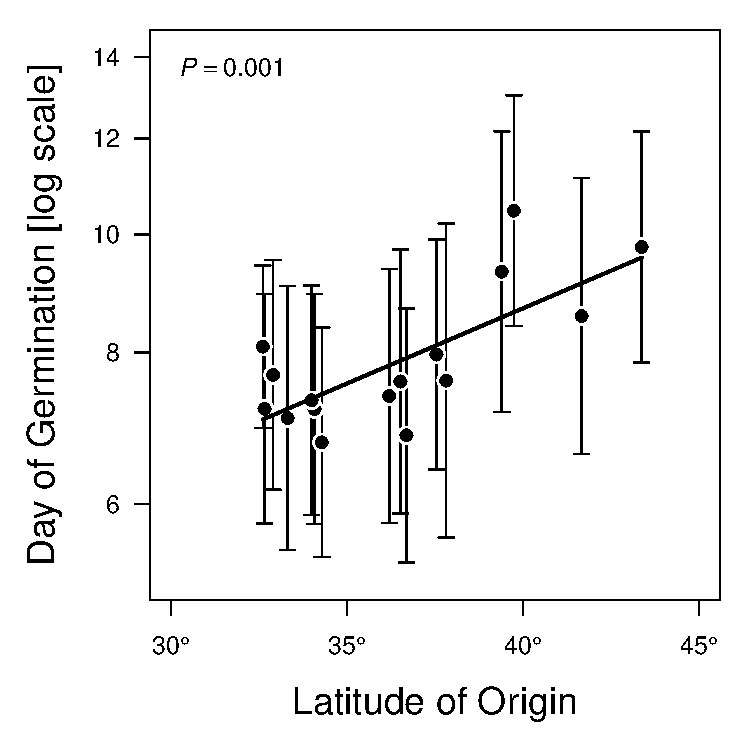
\includegraphics[width=0.5\textwidth]{Figures/Figure_DoG_Lat.pdf}}
	\usefont{T1}{phv}{m}{n}
	\fontsize{10}{12}
	\selectfont
	\caption[Southern populations germinate sooner.]{CAPTION}
	\label{fig:Fig_DoG}
\end{figure}

\begin{figure}[h!]
	\centerline{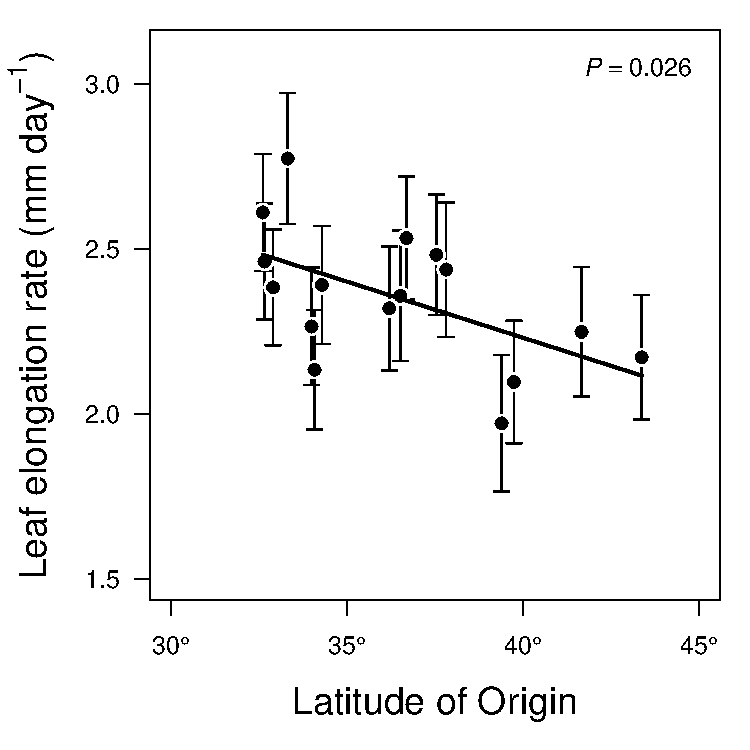
\includegraphics[width=0.5\textwidth]{Figures/Figure_LLL_Lat.pdf}}
	\usefont{T1}{phv}{m}{n}
	\fontsize{10}{12}
	\selectfont
	\caption[Southern populations grow faster (leaf expansion rate).]{CAPTION}
	\label{fig:Fig_LLL}
\end{figure}

\begin{figure}
	\centerline{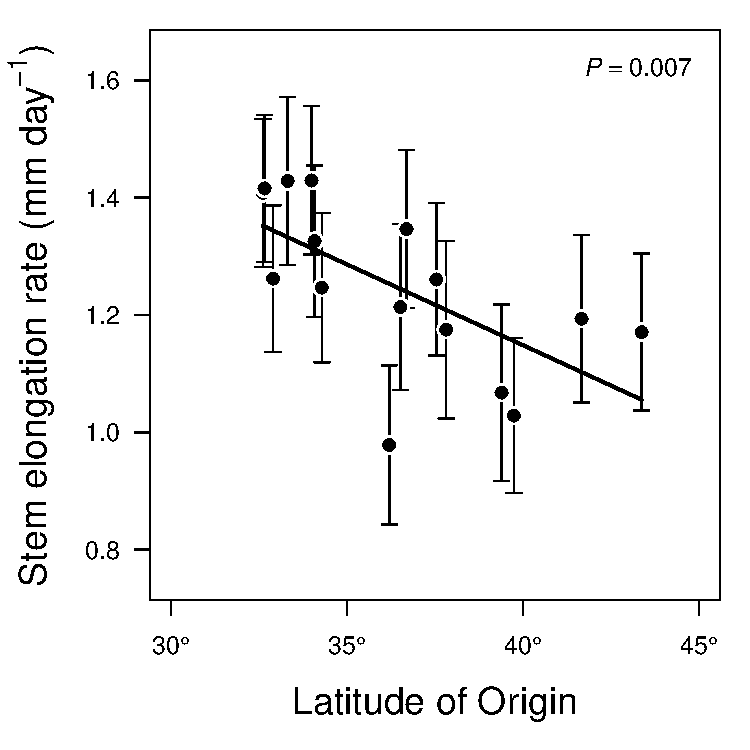
\includegraphics[width=0.5\textwidth]{Figures/Figure_Height_Lat.pdf}}
	\usefont{T1}{phv}{m}{n}
	\fontsize{10}{12}
	\selectfont
	\caption[Southern populations grow faster (stem elongation rate).]{CAPTION}
	\label{fig:Fig_height}
\end{figure}

%--------------------------------------------------
% References
%--------------------------------------------------

\setlength{\bibsep}{6pt}
\bigskip

\bibliography{refs}
\bibliographystyle{evolution}

%--------------------------------------------------
% Supplementary Information
%--------------------------------------------------

% DIC table for initial size (LLL on 5/12)
\begin{table}[htbp]
	\usefont{T1}{phv}{m}{n}
	\fontsize{10}{12}
	\selectfont
	\caption[ANOVA table, leaf expansion rate]{Initial size of seedlings did not vary among Populations, Families, or Treatments. We used a censored Gaussian model of initial size at the outset of the experiment (longest leaf length of the first true leaves). The model was censored because we could not accurately measure leaves less than 0.25 mm with digital callipers (217 of 702, 30.9\%, were too small). We fit models using a Bayesian MCMC method implemented using the MCMCglmm function with default priors in the R package MCMCglmm version 2.17 \citep{Hadfield_2010}. We estimated the posterior distribution from 1000 samples of an MCMC chain run for $10 ^ 5$ steps after a $10^4$ step burn-in. We step-wise backward elimination procedure to find the best-supported model according to Deviance Information Criterion (DIC).}
	\begin{center}
	\begin{tabular}{>{\everypar{\hangindent1cm}{}\raggedright}p{6cm}lc}
	\toprule

	\input{Tables/Table_InitialSize.txt}

	\bottomrule
	\end{tabular}
	\end{center}
\end{table}

\end{document}


	\subsection{Structure}

	Leaf traits method: \\
	Day 1: \\
	- select focal leaf (e.g. second or third leaf); \\
	- place in H20, dark, cool overnight. \\
	Day 2: \\
	- wet weight; \\
	- scan; \\
	- place in drying oven. \\

		\begin{enumerate}
			\item{Stomatal density, guard cell length, ratio from leaf opposite focal leaf (above}
			\item{Leaf size/shape (from scans)}
			\item{Leaf thickness/SLA}
			\item{Colorimetry (from scans, spec)}
			\item{stem anthocyanin (qualitative)}
		\end{enumerate}

	OPEN QUESTIONS: \\
	save wet samples in preservative (e.g. for leaf venation?) \\
	chlorophyll content? \\
	branching architecture (anything in plant protocols?)

	\subsection{Function}

		\subsubsection{during experiment}

		\begin{enumerate}
			\item{Instantaneous photosynthetic rate, $g_\text{s}$, water-use efficiency.}
				\subitem{3 min per plant per LICOR}
				\subitem{Do as many plants as possible in 1-2 weeks}
				\subitem{Before and after drought?}
			\item{Respiration}
			\item{Whole plant water-use (gravimetric)}
				\subitem{}
			\item{Leaf temperature (subset)}
			\item{Temperature response curve (subset)}
				\subitem{see protocol here: http://prometheuswiki.publish.csiro.au/tiki-index.php?page=Temperature+response+of+photosynthesis+using+a+Li-Cor+6400}
			\item{Light response curve}
				\subitem{Sampling? Only in cool, wet?}
				\subitem{At what temperature?}

		\end{enumerate}

		\subsubsection{after experiment}

		\begin{enumerate}
			\item{CN content}
			\item{carbon isotope discrimination}
		\end{enumerate}


	\subsection{Development time and Life history}

	\begin{enumerate}
		\item{Flowering time: census daily}
		\item{Starch accumulation: collect (subset) of plants}
		\item{Rhizome formation: collect on subset of plants harvested for dry mass}
	\end{enumerate}

	\subsection{Floral (2nd/3rd/etc flower?)}

	\begin{enumerate}
		\item{Flower size}
		\item{Herkogamy}
	\end{enumerate}

\section{Performance}

	Possibilities: \\
	1. (sub-)weekly census of plant height. $\approx$ 0.5 min per plant, so allow 1 day \\

	$$RGR_\text{height} = \frac{\text{ln} H_2 - \text{ln} H_1}{t_2 - t_1}$$

	2. early development (pre-treatment) leaf-area growth with camera \\
	3. harvest dry biomass before and after treatments (get whole plant leaf area using scanner at same time to ground truth camera)

	$$RGR_\text{mass} = \frac{\text{ln} M_2 - \text{ln} M_1}{t_2 - t_1}$$

\section{Determining ecological gradients that matter}

Performance tradeoffs
Isolation by ecology

\section{Tests of divergent selection}

	\subsection{Trait-environment correlation}

	We will account for relatedness by using genetic distance matrix in linear models.

	\subsection{$P_\text{ST}$ -- $F_\text{ST}$}

	Contrast trait classes with Fst distribution

	\subsection{Isolation by ecology}

	Is \textbf{G} better predicted by \textbf{E} than geographic distance? Use Gideon's method?

	\subsection{Performance tradeoffs between treatments}


\section{Ecological strategy, physiological mechanism, and tradeoff}

	\subsection{Drought escape}
		Pattern: \\
			Flowering time shorter in drier/S populations \\
			More between population variation in flowering time more variable than predicted by Fst \\
			... \\

	\subsection{Drought avoidance}
		Pattern: \\
			Maybe this should really be dehydration avoidance? \\
			Populations from drier/S avoid dehydration by limiting water loss; more variable than predicted by Fst \\

			Mechanism \\
			closing stomata earlier during soil drying

		Mechanisms: \\
			lower water-use \\

	\subsection{Drought tolerance}
		Pattern: \\
			drier/S populations have greater tolerance to low tissue water content

		Mechanisms: \\
			greater WUE \\
			ability to photosynthesize during drought \\

\section{Extension: incipient speciation as a byproduct or divergence?}

Collect pollen to measure viability.


\end{document}
